\documentclass[letterpaper, 12pt]{article}


\usepackage{parskip,xspace}
\usepackage{amsmath,amsthm,amsfonts,amssymb}
\usepackage{mathrsfs} 
\usepackage{caption}
\usepackage{xcolor} 
\usepackage{geometry}
\usepackage{fancyhdr}
\usepackage{rotating}
\usepackage{multirow}
\usepackage{makecell}
\usepackage{ltxtable}
\usepackage{hyperref}
\usepackage{graphicx}
\usepackage{subfigure}
\usepackage{bm}
\usepackage{listings}
\usepackage[]{statrep}
\usepackage{enumerate}
\usepackage{subfigure}
\graphicspath{{eps/}}


\newcommand{\ba}{$$\begin{aligned}}
\newcommand{\ea}{\end{aligned}$$}
\newcommand{\dx}{\mathrm{d}x}

\lstset{
  language=R,
  basicstyle=\small,
  numbers=left,
  keywordstyle=\color{blue},
  numberstyle={\tiny\color{lightgray}},
  stepnumber=1, %?????????
  numbersep=5pt,
  backgroundcolor=\color[rgb]{0.95,1.0,1.0},
  showspaces=false,
  showtabs=false,
  frame=shadowbox, rulesepcolor=\color{red!20!green!20!blue!20!},
% frame=single,
% TABframe=single,
  tabsize=4,
  breaklines=tr,
  extendedchars=false %???????????????????????????????
}





\pagestyle{fancy}
\lhead{Peng Shao 14221765}
\chead{}
\rhead{\bfseries STAT 8320 Spring 2015 Assignment 3}
\renewcommand{\headrulewidth}{0.4 pt}
\setlength{\parindent}{2em}

\begin{document}
\title{STAT 8320 Spring 2015 Assignment 3}
\author{Peng Shao 14221765}
\maketitle
\indent




$\blacktriangleright$ \textbf{1.\quad Solution.} 
(a). Because $f(y)=\binom{y+k-1}{k-1}p^k(1-p)^y$, then
$$
f(y)=\exp\left\{y\log(1-p)-(-k\log p)+\log\binom{y+k-1}{k-1}\right\}
$$
Let $\theta=\log(1-p)$, then $p=1-e^\theta$. Thus,
\ba
b(\theta)&=-k\log p=-k \log(1-e^\theta)\\
E(Y)&=b'(\theta)=k\frac{e^\theta}{1-e^\theta}=k\frac{1-p}{p}=\mu\\
var(Y)&=b''(\theta)=k\frac{1-p}{p^2}=k\frac{p-p^2+1-2p+p^2}{p^2}\\
&=k\frac{1-p}{p}+k\frac{(1-p)^2}{p^2}=\mu+\frac{\mu^2}{k}\\
\theta&=\log(1-p)\\
a(\phi)&=1\\
c(y,\phi)&=\log\binom{y+k-1}{k-1}
\ea



(b). Because $\mu=E(Y)=k\frac{\exp\{\theta\}}{1-\exp\{\theta\}}$, then
\ba
\mu-\mu e^\theta&=ke^\theta\\
\mu&=(k+\mu)e^\theta\\
e^\theta&=\frac{\mu}{k+\mu}\\
\theta&=\log \frac{\mu}{k+\mu}
\ea
Thus, the canonical link is $\log (\mu/(k+\mu))$



  
(c). \ba
D&=2\sum_{i=1}^{n}(\log f(y_i,\tilde{\theta}_i)-\log f(y_i,\hat{\theta}_i)-(b(\tilde{\theta}_i)-b(\hat{\theta}_i)))\\
&=2\sum_{i=1}^{n}\left(y_i(\tilde{\theta}-\hat{\theta})+k\log\frac{1-e^{\tilde{\theta}_i}}{1-e^{\hat{\theta}_i}}\right)\\
&=2\sum_{i=1}^{n}\left(y_i(\log\frac{y_i}{k+y_i}-\log\frac{\hat{\mu}_i}{k+\hat{\mu}_i})+k\log\frac{k/(k+y_i)}{k/(k+\hat{\mu}_i)}\right)\\
&=2\sum_{i=1}^{n}\left(y_i\log\frac{y_ik+y_i\hat{\mu_i}}{\hat{\mu_i}k+\hat{\mu_i}y_i}+k\log\frac{k+\hat{\mu}_i}{k+y_i}\right)
\ea

(d). Because
\ba
\frac{\partial \ell(\beta_i)}{\partial \theta_i}&=y_i-\mu_i\\
\frac{\partial \theta_i}{\partial \mu_i}&=\frac{k}{\mu^2+k\mu}\\
\frac{\partial \mu_i}{\partial \eta_i}&=\mu_i\\
\frac{\partial \eta_i}{\partial \beta_j}&=x_{ij}
\ea
Then
$$
\frac{\partial \ell(\beta)}{\beta_j}=\sum_{i=1}^{n}\frac{\partial \ell(\beta_i)}{\partial \theta_i}\frac{\partial \theta_i}{\partial \mu_i}\frac{\partial \mu_i}{\partial \eta_i}\frac{\partial \eta_i}{\partial \beta_j}=\sum_{i=1}^{n}\frac{k(y_i-\mu_i)}{(k+\mu_i)}x_{ij}
$$

(e).Because
\ba
V(\mu_i)&=\frac{k\mu_i+\mu_i^2}{k}\\
\frac{\partial \eta_i}{\partial \mu_i}&=\frac{1}{\mu_i}
a(\phi)&=1
\ea
then
$$
w_i=\left\{\left(\frac{\partial \eta_i}{\partial \mu_i}\right)^2V(\mu_i)\right\}^{-1}=\frac{k\mu_i}{k+\mu_i}
$$
Thus, the $(j,k)$th element of the Fisher information matrix is equal to
$$
\sum_{i=1}^{n}\frac{w_i}{a(\phi)}x_{ij}x_{ik}=\sum_{i=1}^{n}\frac{\mu_ik}{k+\mu_i}x_{ij}x_{ik}
$$

(f)
\ba
\bm{\hat{\beta}^{(1)}}&=\left(\begin{array}{c c c}0.2047 & 1.3520 & 0.0435\end{array}\right)'\\
\bm{F}&=\frac{\partial\bm{\mu}}{\partial\bm{\beta}}=(\mu_i\cdot x_{ij})_{7\times3}\\
&=\left(\begin{array}{c c c c c c c}9.1157 & 4.3060 & 7.0287  & 11.2459 & 4.9530 & 6.8895 & 6.5535\\
0 & 4.3060 & 7.0287 &   0 & 4.9530 &  0 & 6.5535\\
319.0501 & 258.3576 & 175.7172 & 224.9172 & 247.6516 & 378.9231 & 196.6051\end{array}\right)'\\
\bm{V}&=\left(\begin{array}{c c c c c c c}
14.6555\\
&5.5420\\
&&10.3222\\
&&&19.6771\\ 
&&&&6.5885\\
&&&&&10.0539 \\
&&&&&&9.4167\end{array}\right).\\
\bm{\mu}&=\left(\begin{array}{c c c c c c c}9.1157 & 4.3060 & 7.0287 &  11.2459 & 4.9530 & 6.8895 & 6.5535\end{array}\right)' 
\ea
The hypotheses are
$$
H_0:~\left(\begin{array}{c c c}
0&1&0\\
0&0&1\end{array}\right)\bm{\beta}=\left(\begin{array}{c c}0&0\end{array}\right)'\quad\text{v.s.}\quad H_a:~\text{Either $\beta_1$ or $\beta_2$ not equal zero}
$$
Then
\ba
\bm{L}&=\left(\begin{array}{c c c}
0&1& 0\\
0&0&1\end{array}\right)\\
\bm{d}&=\left(\begin{array}{c c}0&0\end{array}\right)'\\
W&=(\bm{L}\bm{\hat{\beta}}-\bm{d})'(a(\phi)\bm{L}(\bm{\hat{F}}'\bm{\hat{V}}^{-1}\bm{\hat{F}})^{-1}\bm{L}')^{-1}(\bm{L}\bm{\hat{\beta}}-\bm{d})=3.0477\\
\text{Pr}(>W)&=0.2178715
\ea
Thus, we failed to reject the null hypothesis, that is, $\beta_1=\beta_2=0$.
However this conclusion is untenable since the $\bm{\hat{\beta}^{(0)}}$ is a very poor and biased estimate of $\bm{\beta}$. If we use the converged estimates of parameters, then we can get $W=15.90$ with P-value=0.0004, which means that we should reject the null hypothesis, i.e., at least one of the parameters are not equal to zero.


(g) In the case, the model can by constructed as before, where $Y_i$ is the number of days absent. The parameter $k$ may likely be number of days attending, by comparing the form of binomial coefficient. Then we put this model and null model into SAS.
\begin{Sascode}
proc genmod data = da.h3q1;
model daysabs = male math langarts /dist=negbin;
run;
proc genmod data = da.h3q1;
model daysabs = / dist=negbin;
run;
quit;
\end{Sascode}

From the output, we know that The log likelihood for the full model is -880.8731 and is -891.2427 for the null model. Then the hypotheses are
$$
H_0:~\text{null model}\quad\text{v.s.}\quad H_a:~\text{full model}
$$
The statistic is
$$
\bm{\wedge}=2(\ell(full~model)-\ell(null~model))=2\times( -880.8731 - -891.2427) = 20.7392
$$
Since we have three predictor variables in the full model, the degrees of freedom for the chi-squared test is 3. This yields a P-value =0.0001192552. Thus, our  model is statistically significant. We also should notice that the estimate of coefficient of "math" is not significant, i.e., "math" may have no effect on predictions of days of absent.

Secondly we estimate the dispersion parameter. From SAS, the estimate of dispersion is 1.2884, which is the estimate of $1/k$. We should get the expectation of $k$, then compare the dispersion parameter estimate to it. As we define before, the $k$ is the number of days attending, and this number should much larger than 1. So $1/k$ should be less than 1. Thus the data is overdispersion. One of the reasons of it is that the parameter $k$ is not a constant number, and the variation of $k$ will cause more variation of $Y$.

\Listing[store=class,
         caption={Estimate Summary}]{h3re5a}
         
         
Finally, we will interpret the parameters (Figure \ref{h3re5a}): 
\begin{enumerate}

\item the estimate of intercept here means that for females (the variable male evaluated at zero) with zero math and langarts test scores, the log of the expected count for daysabs is 2.7161 units. Since that zero scores are meaningless, the interpretation will be more reasonable if we would have a little change: we let math and langarts be centralized, then the intercept would have a natural interpretation: the log of the expected count for females with average mathnce and langnce test scores.

\item The difference in the logs of expected days absent is expected to be 0.4312 unit lower for males compared to females, while holding the other variables constant in the model.

\item If a student were to increase her langnce test score by one point, the difference in the logs of expected counts would be expected to decrease by 0.0143 unit while holding the other variables in the model constant.

\item If a student were to increase her mathnce test score by one point, the difference in the logs of expected counts would be expected to decrease by 0.0016 unit, while holding the other variables in the model constant. (Reference from \textit{SAS Annotated Output}, IDRE)
\end{enumerate}

$\blacktriangleright$ \textbf{2.\quad Solution.} 
(a). Because $Y\sim \text{BIN}(50,p_{i})$,where $p_i$ is the rate of germination, we consider a Binomial Regression Model. Then
$$
f(y_i;50,p_i)=\binom{50}{y_i}p_i^{y_i}(1-p_i)^{50-y_i}
$$
The exponential form of probability mass function is
$$
f(y_i;\theta, \phi)=\exp\left[\frac{\theta_iy_i-b(\theta_i)}{a(\phi)}+c(y_i,\phi)\right]
$$
where
\begin{itemize}
\item $\theta_i=\text{logit}(p_i)=\log\left(\frac{p_i}{1-p_i}\right)$
\item $b(\theta)=50\log(1+e^\theta)$
\item $a(\phi)=1$
\item $c(y_i,\phi)=\log\binom{50}{y_i}$
\end{itemize}
This is the random component of the model. 

Since $y_i$ can be treated as a grouped Bernoulli variable, the link function is 
$$
\eta_i=g(p_i)=\text{logit}(p_i)=\log\left(\frac{p_i}{1-p_i}\right)
$$
where $\eta_i$ is linear predictor.

Because there are two factor and 4 levels for each, the linear predictor is
$$
\eta_i=\mu+\sum_{j=1}^{3}\beta_jX_{ij}+\sum_{k=1}^{3}\gamma_kZ_{ik}+\sum_{j=1}^{3}\sum_{k=1}^{3}\delta_{jk}X_{ij}Z_{ik}
$$
where
\begin{itemize}
\item $X_{ij}=1$, if $j$th level of temperature; $X_{ij}=-1$, if 4th level of temperature; otherwise $X_{ij}=0$.
\item $Z_{ik}=1$, if $k$th level of concentration; $Z_{ik}=-1$, if 4th level of temperature; otherwise $Z_{ik}=0$.
\end{itemize}
The link function and the linear predictor is the systematic component of the model.


(b) Yes. The degree of freedom of model 4 is 57, and the degree of freedom of model 5 is 48. The hypotheses are
$$
H_0:~\text{model 4}\quad\text{v.s.}\quad H_a:~\text{model 5}
$$
Because 
$$
T=\frac{D(model~4)-D(model~5)}{\phi}=\frac{148.1-55.6}{1}=92.5>\chi^2_{0.95,57-48}=16.92
$$
then we reject $H_0$, that is, the interaction term is needed in the model.


(c) The hypotheses are
$$
H_0:~\text{model 5 is good enough to fit data}\quad\text{v.s.}\quad H_a:~\text{model 5 is lack of fit}
$$
The statistic is
$$
D^*=2(\ell(saturated~model)-\ell(model~5))=D(model~5)=55.6<\chi^2_{0.95,64-16}=65.17077
$$
Thus, we fail to reject null hypothesis, i.e., the mode 5 is good enough to fit data. In addition, the dispersion parameter is $\phi=55.6/48=1.158$, which is very close to 1, so the binomial model is appropriate.

To sum up, there is no significant evidence of lack of fit for model 5.


(d) Because
\ba
\text{logit}(\hat{p}_{X_1+1})-\text{logit}(\hat{p}_{X_1})&=\beta_0+\beta_1X_1+\beta_2X_2+\beta_3X_1X_2\\
&-\beta_0+\beta_1(X_1+1)+\beta_2X_2+\beta_3(X_1+1)X_2\\
&=\beta_1+\beta_3X_2
\ea
Then the odds ratio for $X_1$ is 
$$
\frac{\text{odds}[\hat{p}_{X_1+1}]}{\text{odds}[\hat{p}_{X_1}]}=e^{\beta_1+\beta_3X_2}
$$

The $\exp(\beta_1)$ here is that the odds ratio for $X_1$ when $X_2$ equals zero, while $\exp(\beta_1)$ in the models without interaction means odds ratio for $X_1$ just holding $X_2$ unchanged. So the meaning is different.

\begin{figure}[htbp]
  \centering
  \caption{Boxplots of Independent Variables v.s. mpg01}\label{boxplot}
  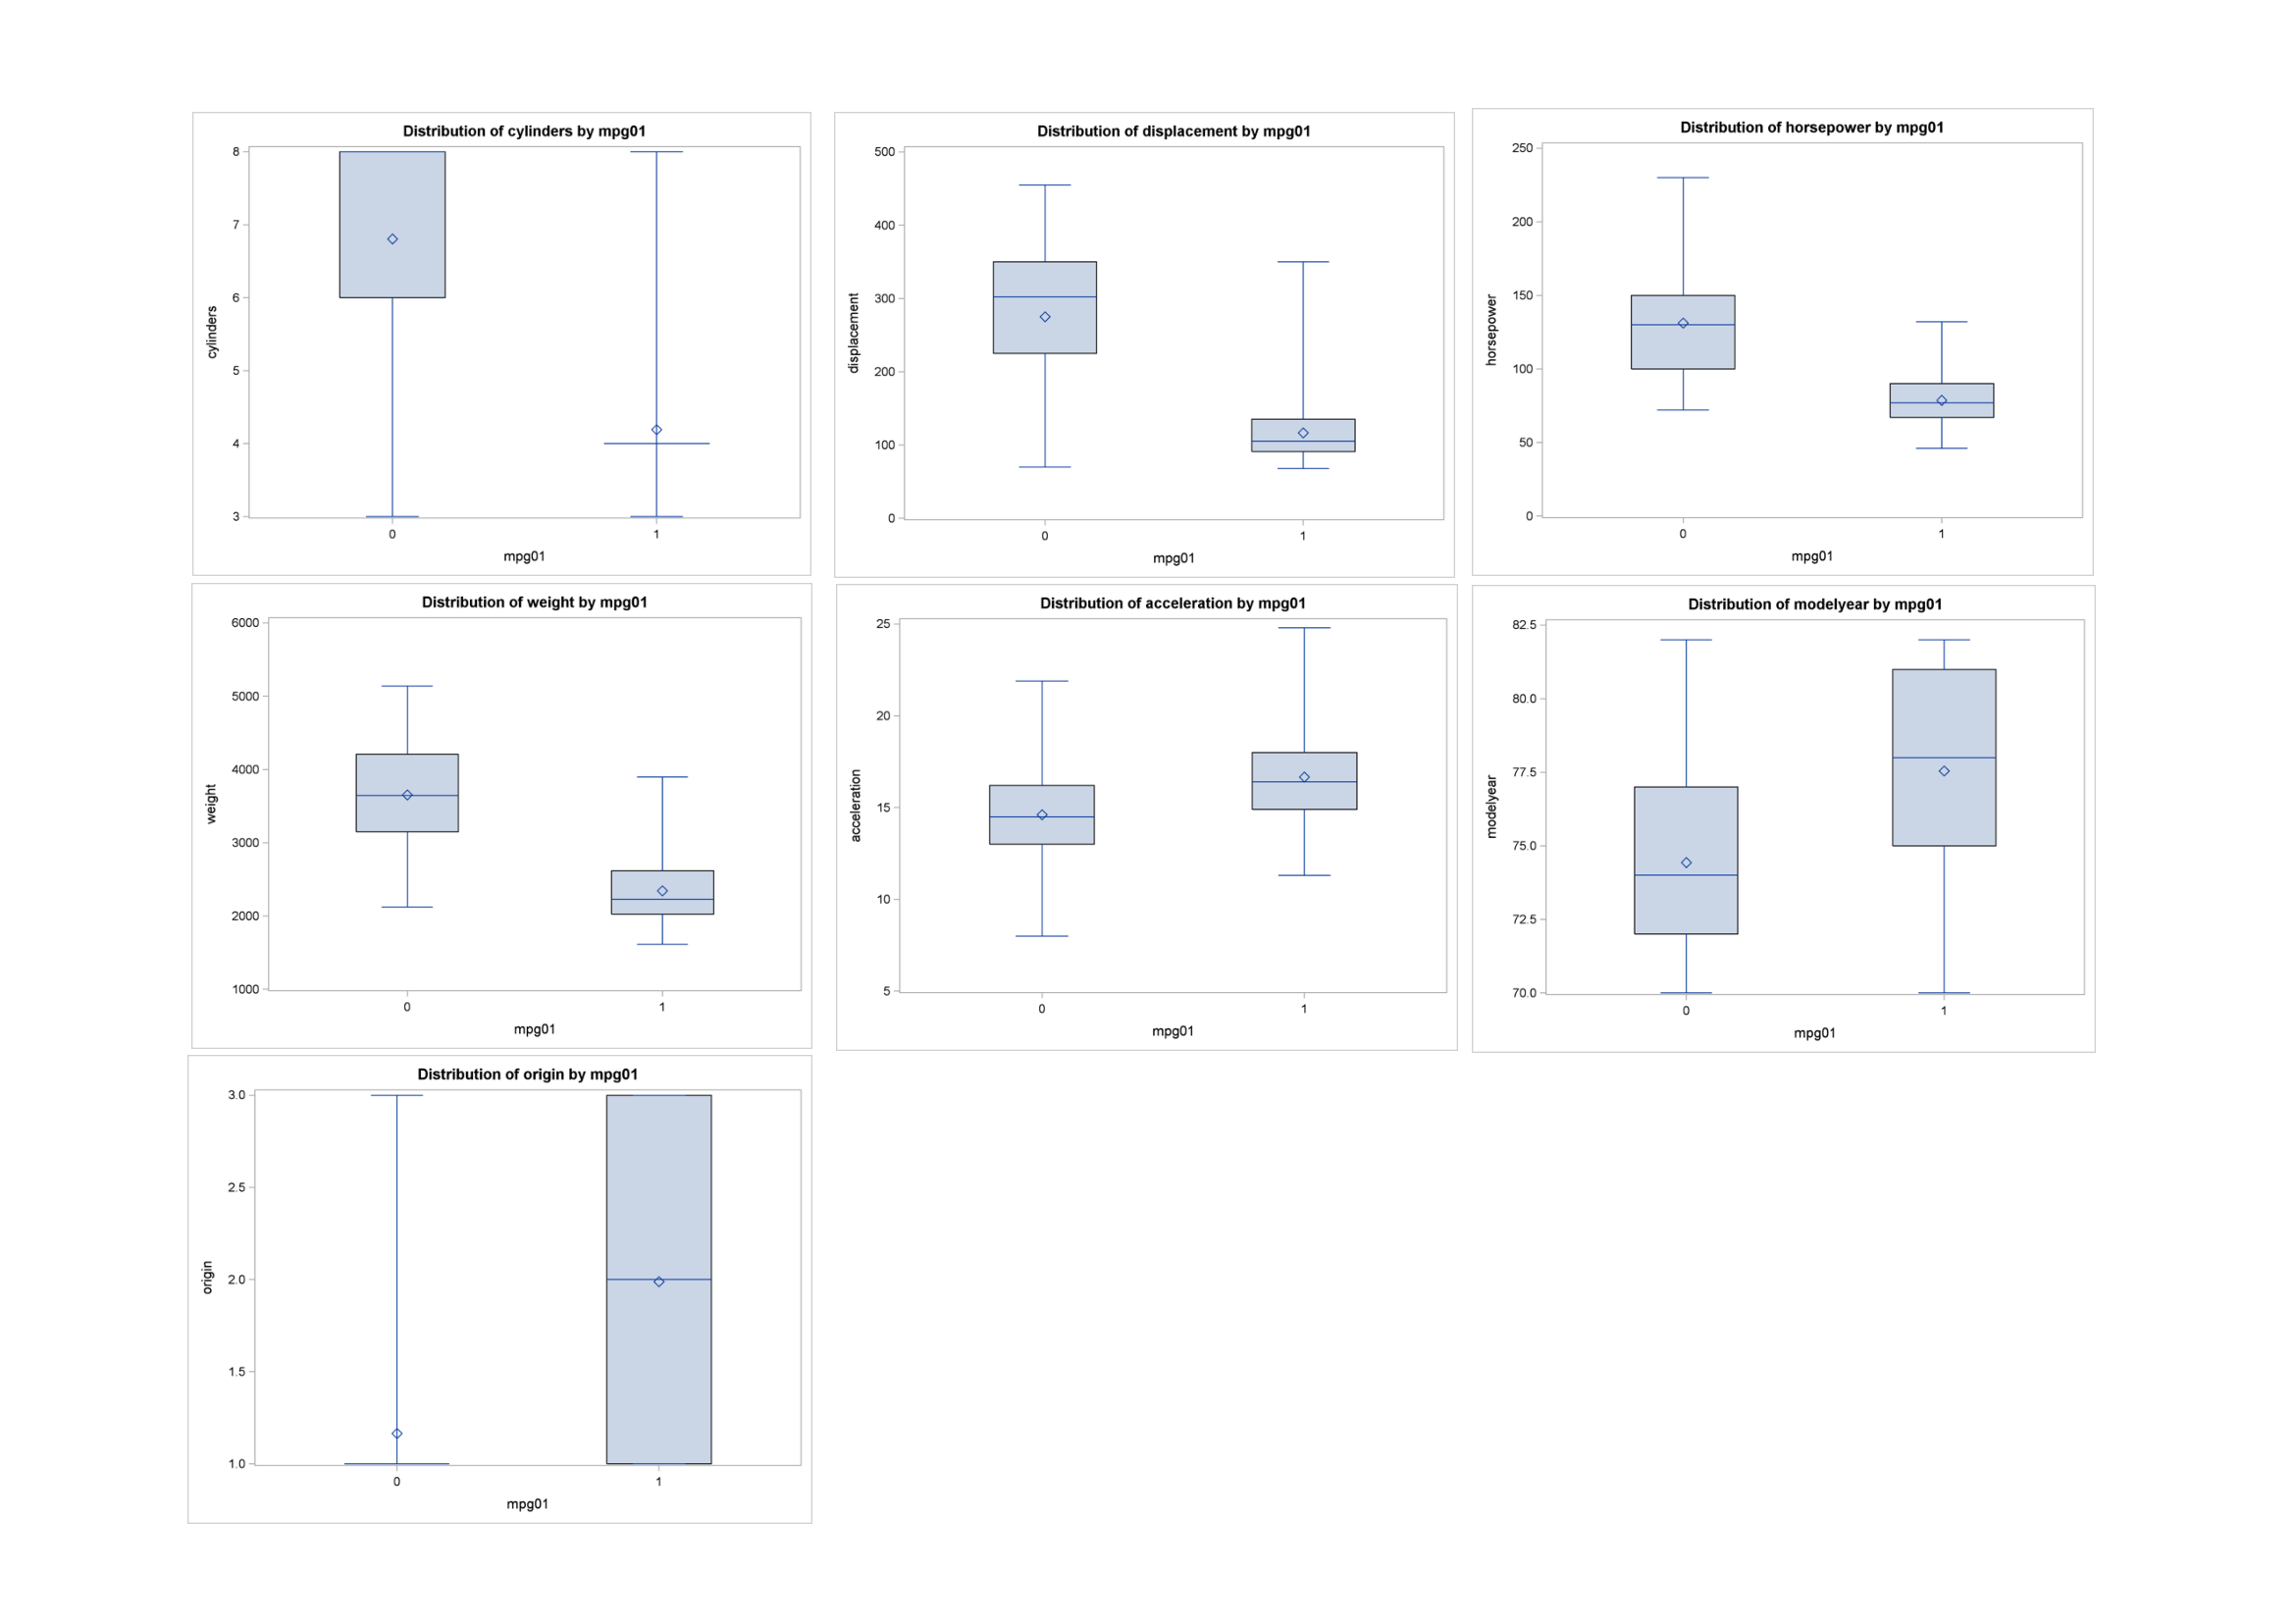
\includegraphics[width=\textwidth]{boxplots.pdf}
\end{figure}

$\blacktriangleright$ \textbf{3.\quad Solution.} 


(a). From the scatterplots (Figure.\ref{scatter}), we can see that the displacement, horsepower, weight and acceleration seem to have effects the level of gas milage because most one of mpg01 distributed in low level of displacement, horsepower and weight, or the high level of acceleration. But these variables have some multicollinearity, so maybe only one or two variable of them will be selected into the model.

From the boxplots (Figure \ref{boxplot}), the boxes of variable acceleration, model year and origin have some overlap, so this means that these variables may not have significant effects on the gas milage, then they may not be selected into the models.

That is all that can be found from the plots.

\Graphic[store=class, scale=0.6,
         caption={Scatterplots of Variables}]{scatter}
(b). Since we do not have too may variables, just to be safe, I will ignore the results from part(a), and still treat all independent variables as potential predictors to select the appropriate ones. I use the 'selection=' option of model statement to preform a predictor selection, as the code below,
\begin{Sascode}[store=class]
PROC LOGISTIC DATA=q31 DESCENDING;
class cylinders modelyear origin;
MODEL mpg01=cylinders displacement horsepower weight
 acceleration modelyear origin/selection=stepwise;
RUN;
\end{Sascode}
where I treat "cylinders", "modeler" and "origin" as indictor variables. The variable of selection result is \{cylinders, modelyear, weight\}, which is inn accordence with what we got from part(a), except "modelyear" becoming a significant predictor. So the model becomes 
$$
Model~1:~Gas~Mileage=Overallmean+Weight+Cylinder+Modelyear
$$
with the 17 parameters (Figure \ref{h3re34}).
\Listing[store=class,
         caption={Predictors Selected}]{h3re34}

Then I score the training dataset under this model, the result shows that the error rate is only 5.56\%, so I have to say that it is really a good prediction model. But I still try the other models,
\ba
Model~2&:~Gas~Mileage=Overallmean+Weight+Cylinder+Modelyear+Interaction\\
Model~3&:~Gas~Mileage=Overallmean+Weight+Cylinder\\
Model~4&:~Gas~Mileage=Overallmean+Weight+Horsepower+Modelyear\\
\ea

Here, Model 2 extends Model 1 by adding interaction; Model 3 drop the variable model year, since we did not want to consider this variable from part(a); and Model 4 is obtained from model selection procedure without treating discrete variables as indicator variables (which may make the model hard to interpret). 
\Listing[store=class,
         caption={Score for Training Dataset}]{h3re38}

I scored data under different models. Model 4 and Model 3 has worse performance in predicting, with the error rates about 10\% and 12\% respectively. So compared to Model 1, they cannot be better model. Model 2, however, has a little lower error rate about 4\%, which improves Model 1 slightly. But Model 2 has two problems: 1) the number of parameters become 57. This may cause model overfitted the data because of two many variable. The decision boundary of the model becomes more complicated and make the prediction for new data more uncertain; 2) the interaction term is very hard to be interpreted. For example, it may be a little difficult to understand than why the number of cylinders has some interaction with model year. Thus, I prefer the Model 1 to be the best model for this problem

The confusion matrix of this model is Figure \ref{h3re39}. Then
\ba
TP=160,\quad FN=11,\quad FP=8,\quad TN=163
\ea
\ba
\text{sensitivity}&=\frac{TP}{TP+FN}=\frac{160}{160+11}=93.57\%\\
\text{specificity}&=\frac{TN}{TN+FP}=\frac{163}{163+8}=95.32\%
\ea
\ba
\text{Type I error}&=\frac{FP}{TN+FP}=\frac{8}{163+8}=4.68\%\\
\text{Type II error}&=\frac{FN}{TP+FN}=\frac{11}{160+11}=6.43\%
\ea
The sensitivity and specificity are both very good, which means that the model has a good ability to determine high and low gas mileage.
\Listing[store=class,
         caption={Confusion Table for Training Dataset}]{h3re39}


Finally, the deviance of this model is 90.7560 with the degree of freedom 318 (Figure \ref{h3re31}), so the dispersion parameter is 0.2854. The assumption of this model is the data follows Bernoulli distribution, i.e., $\phi$ equals 1. Thus there is much less variation than we expected.
\Listing[store=class,
         caption={Model Fitness Summary}]{h3re31}

(c) The code here is 
\begin{Sascode}[store=class]
PROC LOGISTIC DATA=q31 DESCENDING outmodel=model;
class cylinders modelyear origin;
MODEL mpg01=cylinders weight modelyear/ scale=none AGGREGATE;
score data=q31 out=score fitstat;
RUN;
PROC LOGISTIC inmodel=model;
score data=q3t1 out=Scoret fitstat;
RUN;
proc freq data=scoret;
tables F_mpg01* I_mpg01/nocol nocum norow nopercent;
run;
\end{Sascode}

The output are listed as below (Figure \ref{h3re40} and Figure \ref{h3re41}). The overall error rate is 10\%. From the confusion matrix (Figure \ref{h3re41}), the sensitivity is 83\%, and specificity is 96.15\%, they are both good, and the ability of determining low gas mileage of this model is better than that of determining high gas mileage.
\Listing[store=class,
         caption={Score for Test Dataset}]{h3re40}
\Listing[store=class,
         caption={Confusion for Test Dataset}]{h3re41}



$\blacktriangleright$ \textbf{4.\quad Solution.} 
(a) We consider a Poisson regression model. The random component of this model is 
$$
f(y;\theta,\phi)=\exp\left\{\frac{y\theta-e^\theta}{\phi}+c(y,\phi)\right\}
$$
the link function is 
$$
g(\mu)=\log(\mu)=\eta
$$
and the linear predictor is
$$
\eta=\beta_0+\beta_1X_1+\beta_2X_2+\beta_3X_3
$$
where $Y$ is fish count and $X_{i}=1$, if $i$th macrohabitat; otherwise $X_{i}=0$. 

From SAS output (Figure \ref{h3re47}), firstly because the type 1 and type 3 analysis is significant, which means that the factor microhabitat has significant effect. Then we study on the estimate summary table. The intercept is the estimate of the effect of macrohabitat 4, the $\beta_i$s are the difference between the effect of macrohabitat $i$ and the effect of macrohabitat 4. Because the estimates of $\beta_i$s are all greater than 0, we can know that the effects of macrohabitat 1,2 and 3 are all greater than that of 4, and the order is $macrohabitat ~1>macrohabitat ~2>macrohabitat ~3>macrohabitat ~4$. Then since the P-value of the estimate of $\beta_2$ is greater than 0.05, there is no significance difference between macrohabitat 2 and macrohabitat 4, which also means no significance difference between macrohabitat 2 and macrohabitat 3 or macrohabitat 3 and macrohabitat 4. However, the P-value of the estimate of $\beta_1$ is less than 0.05, which means that there is a significance difference between macrohabitat 1 and macrohabitat 4. Actually, we can construct the models under other coding schemes like reference to "1" for indicator variables, and we can get to know that the significance difference is only between macrohabitat 1 and macrohabitat 4, while there is no significant differences between any other pair of macrohabitats.
\Listing[store=class,
         caption={Estimate Summary}]{h3re47}

The dispersion parameter is 9.8390, which is much greater than 1. It implies that the data is over dispersion based on this Poisson model. This makes us to think about other models like Extra-Poisson model or zero inflated Poisson model to fix this problem.


(b). Because of the excess of zero (Figure \ref{h3re9}), we consider the zero-inflated Poisson model,
$$
f(y)=\left\{\begin{array}{l l}\omega+(1-\omega)e^{-\lambda}\qquad &\text{for }y=0\\
(1-\omega)\frac{\lambda^ye^{-\lambda}}{y!}\qquad &\text{for }y=1,2,...
\end{array}\right.
$$
and
\ba
h(\omega_i)&=\bm{z_i}\bm{\gamma}\\
g(\lambda_i)&=\bm{x_i}\bm{\beta}
\ea

In this problem, $h(\cdot)$ is logit function, $g(\cdot)$ is log function, $X$ is macrohabitat, and $Z$ is gear type. Here, the macrohabitat is treated as count portion of the model, and the gear type is treated as zero-inflation portion in this model. From the output, we can see that P-values of estimates of $\gamma_3$ an $\gamma_5$ are less that 0.05, which means that type 2 gear and type 4 gear are significantly different from type 5 gear, so we can think that gear type has a significant effect, or we can say the zero-inflated model is significantly better that the pure Poisson regression model. We can also perform a Vuong test (Figure \ref{h3re66}, since these two are not nested models which can be tested by full-reduced model test. From the output, we can see that P-values of three statistics are all less than 0.05, which mean one of the two models is closer to the true model and the test prefer the ZIP model.
\Graphic[store=class, scale=0.6,
         caption={Histogram of Fish Count}]{h3re9}
\Listing[store=class,
         caption={Test Result for ZIP Model}]{h3re66}











%\Listing[store=class,
%  caption={Regression Analysis}]{resultl}

%\Graphic[store=class, scale=0.9,
%  caption={Graphs for Regression Analysis}]{resultg}

\end{document}